\section{Ziel}
\label{sec:Ziel}
Im Folgenden Versuch sollen unbekannte Widerstände, Induktivitäten und Kapazitäten sowie die Frequenzabhängigkeit der Brückenspannung einer Wien-Robinson Brücke bestimmt werden.

\section{Theorie}
\label{sec:Theorie}
Brückenschaltungen dienen zum Ausmessen von Größen, welche sich als elektrischer Widerstand darstellen lassen. Eine Brückenschaltung besteht allgemein aus vier Widerständen und einer Speisespannung.

\begin{figure}
  \centering
  \includegraphics[scale=0.5]{content/Brückenschaltung_prinzipiell.jpg}
  \caption{Prinzipielle Brückenschaltung. Aus \cite{anleitung302}.}
  \label{fig:brückenschaltung}
\end{figure}

Zwischen den Punkten A und B wir eine Potentialdifferenz gemessen, welche Brückenspannung geißt.
Es gelten die Kirchhoffschen Gesetze.
\begin{enumerate}
  \item In einem Knotenpunkt ist die Summe aller Ströme gleich Null.
  \begin{equation}
    \mathrm\sum_{k} I_k = 0
  \end{equation}
  \item In einer abgeschlossenen Masche ist die Summe aller Spannungen gleich Null.
  \begin{equation}
    \mathrm\sum_{k} U_k = 0
  \end{equation}
\end{enumerate}

Daraus folgt für die Brückenspannung:
\begin{equation}
  U_{\mathrm{Br}} = \frac{R_{2}R_3 - R_{1}R_4}{(R_3 + R_4)(R_{1} + R_{2})} U_S .
\end{equation}

Die Brückenspannung geht gegen Null, wenn
\begin{equation}
  R_{1} R_4 = R_{2} R_3 .
\end{equation}
Dies ist die sogenannte Abgleichbedingung.
$R_{1}$ und $R_4$ können sowohl ohmsche als auch komplexe Widerstände sein. Da sich komplexe Widerstände aus einem Wirk- und einem Blindwiderstand  zusammensetzen, werden in den folgenden Unterkapiteln spezielle Brückenschaltungen erläutert.

\subsection{Wheatstonesche Brücke}
\begin{figure}
  \centering
  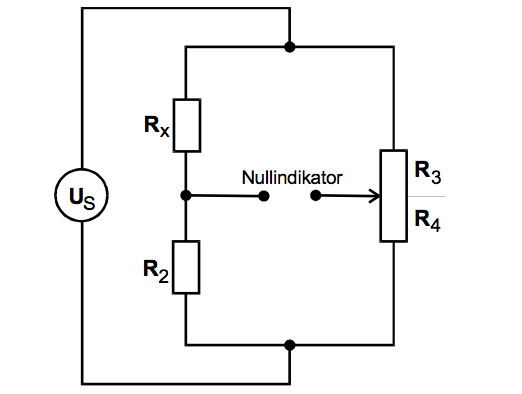
\includegraphics[scale=0.5]{content/wheatstone.jpg}
  \caption{Wheatstonesche Brücke. Aus \cite{anleitung302}.}
  \label{fig:wheatstone}
\end{figure}

Der Widerstand $R_{1}$ in der prinzipiellen Brückenschlatung wird hier durch einen unbekannten Widerstand $R_x$ ersetzt. Für $R_x$ gilt:
\begin{equation}
\label{eqn:wheatstone}
  R_x = R_{2} \frac{R_3}{R_4}.
\end{equation}
Da nur das Verhältnis der Widerstände $R_3$ und $R_4$ zur Berechnung von $R_x$ relevant ist, werden die beiden bekannten Widerstände in einem Potentiometer abgebildet.

\subsection{Kapazitätsmessbrücke}

\begin{figure}
  \centering
  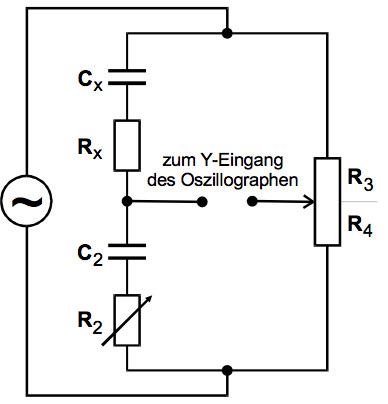
\includegraphics[scale=0.5]{content/kapazitätsbrücke.jpg}
  \caption{Kapazitätsmessbrücke. Aus \cite{anleitung302}.}
  \label{fig:kapazität}
\end{figure}

Zur Messung von Kapzitäten, also komplexen Widerständen, wird die Kapazitätsmessbrücke werwendet. Sie wird wegen der komplexen Widerstände mit Wechselstrom betrieben.
Für reale Kondensatoren gilt für den Widerstand:

\begin{equation}
  \mathfrak{Z}_C = R - \frac{j}{\omega C}
\end{equation}

Da reale Kondensatoren einen Teil der elektrischen Energie in Wärme umwandeln, wird im Schaltbild ein ohmscher Widerstand zur Kapazität in Reihen geschaltet.
Um die durch $R_x$ auftretende Phasenverschiebung zu kompenseiren, wird ein variabler Widerstand $R_{2}$ eingebaut. Für $C_x$ und $R_x$ folgt:

\begin{equation}
  \label{eqn:kapazität1}
  C_x = C_{2} \frac{R_4}{R_3}
\end{equation}
\begin{equation}
  \label{eqn:kapazität2}
  R_x = R_{2} \frac{R_3}{R_4}.
\end{equation}

\subsection{Induktivitätsmessbrücke}

\begin{figure}
  \centering
  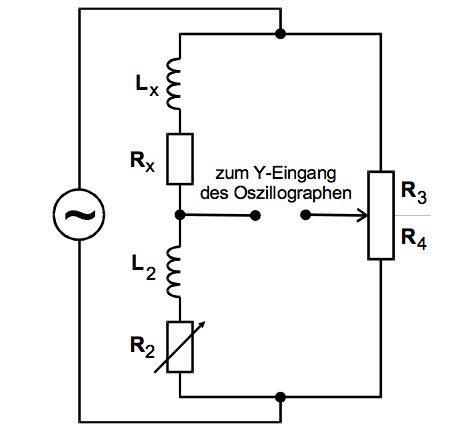
\includegraphics[scale=0.5]{content/induktivitätsmessbrücke.jpg}
  \caption{Induktivitätsmessbrücke. Aus \cite{anleitung302}.}
  \label{fig:induktivität}
\end{figure}

Hier sollen Induktivitäten ausgemessen werden. Da diese ebenfalls komplexe Widerstände sind, ist Wechselstrom zum Betreiben erforderlich.
Der Widerstand einer realen Spule ergubt sich aus

\begin{equation}
  \mathfrak{Z}_L = R + j\omega L
\end{equation}


Eine ideale Spule wandelt einen Teil der magnetischen Feldenergie in Wärme um. Auch ihr Schaltbild enthält zusätzlich einen in Reihe geschalteten ohmschen Widerstand.
Auch hier dient der Widerstand $R_{2}$ dazu, eine Phasenverschiebung, welche durch den Innenwiederstand der Spule verursacht wird, auszugleichen.
Für $L_x$ und $R_x$ gilt:

\begin{equation}
  \label{eqn:ind1}
  L_x = L_{2} \frac{R_3}{R_4}
\end{equation}

\begin{equation}
  \label{eqn:ind2}
  R_x = L_{2} \frac{R_3}{R_4}.
\end{equation}

Für eine möglichst genaue Messung müsste nur $R_{2}$ in diesem Brückenzweig dem Wirkwiderstand entsprechen, was bei niedrigen Frequenzen schwer umzusetzen ist.

\subsection{Maxwell-Brücke}

\begin{figure}
  \centering
  \includegraphics[scale=0.5]{content/maxwell-brücke.jpg}
  \caption{Maxwell-Brücke. Aus \cite{anleitung302}.}
  \label{fig:maxwell}
\end{figure}

Auch die Maxwell-Brücke dient zum Messen von Induktivitäten. Die Widerstände $R_3$ und $R_4$ werden als Abgleichelemente eingebaut. Die Kapazität $C_4$ besitzt einen möglichst geringen Wirkwiderstand. Für $L_x$ und $R_x$ gelten folgende Beziehungen:

\begin{equation}
  \label{eqn:max1}
  L_x = R_{2} R_3 C_4
\end{equation}

\begin{equation}
  \label{eqn:max2}
  R_x = R_{2} \frac {R_3}{R_4}
\end{equation}

\subsection{Wien-Robinson-Brücke}

\begin{figure}
  \centering
  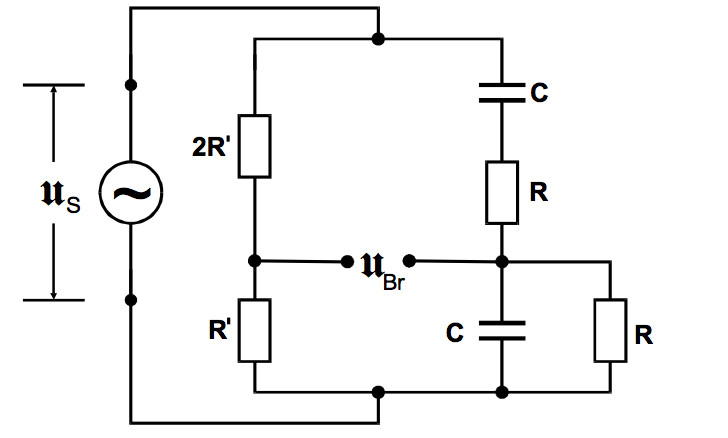
\includegraphics[scale=0.5]{content/wien-robinson.jpg}
  \caption{Wien-Robinson-Brücke. Aus \cite{anleitung302}.}
  \label{fig:wien-robinson}
\end{figure}

Diese Schaltung enthält keine Abgleichelemente. Sie hat die Funktion eines elektronischen Filters, was durch das Spannungsverhältnis von Brücken- und Speisespannung erkennbar ist.


\begin{equation}
\left\lvert\frac{U_\mathrm{Br,eff}}{U_S}\right\rvert^2 = {(\omega^2 R^2 C^2 -1)^2}{9((1 - \omega^2 R^2 C^2)^2 + 9\omega^2 R^2 C^2)}
\end{equation}

Wenn
\begin{equation}
  \label{eqn:resonanz}
  \omega_0 = \frac{1}{RC},
\end{equation} geht die Brückenspannung gegen Null. Frequenzen nahe $\omega_0$ werden abgeschwächt.
Mit $\Omega = \frac{\omega}{\omega_0}$ folgt:

\begin{equation}
  \label{eqn:wr}
  \left\lvert \frac{U_\mathrm{Br,eff}}{U_S} \right\rvert^2 = \frac{1}{9} \frac {(\Omega^2 -1^2)}{(1 - \Omega^2)^2 + 9 \Omega^2}
\end{equation}

\subsection{TT-Brücke}
\begin{figure}
  \centering
  \includegraphics[scale=0.5]{content/TT-Brücke.jpg}
  \caption{TT-Brücke. Aus \cite{anleitung302}.}
  \label{fig:tt}
\end{figure}

Die TT-Brücke hat ebenfalls die Funktion eines elktronischen Filters. Ein Vorteil gegenüber der Wien-Robinson-Brücke besteht darin, dass Eingangs-, Ausgangs- oder Brückenspannung gegen Masse angeschlossen werden können.
Die Ausgangsspannung geht gegen Null, wenn $\omega_0 = \frac{1}{RC}$.
Für die Brückenspannung gilt:

\begin{equation}
  U_\mathrm{Br} = U_S \frac{1 - \omega^2 R^2 C^2}{1 - \omega^2 R^2 C^2 + 4j \omega R C}
\end{equation}

Mit $\Omega = \frac{\omega}{\omega_0}$ und Multiplikation mit dem konjugiert Komplexen gilt:
\begin{equation}
 \left\lvert\frac{U_\mathrm{Br}}{U_S}\right\rvert^2 = \frac{(\omega^2 - 1)^2}{(1 - \omega^2)^2 + 16\omega^2}
\end{equation}

\subsection{Klirrfaktor}
Der Gehalt der Oberwellen im Verhältnis zur Grundwelle des Frequenzgenerators wird durch den Klirrfaktor $k$ berechnet.
\begin{equation}
  \label{eqn:klirr1}
  k = \frac{\sqrt{\sum_{i=2}^N U_i^2}}{U_{1}}
\end{equation}
Unter der Annahme, dass die Oberwellen lediglich aus einer einzigen zusätzlichen Schwingung bestehen lässt sich dies zu
\begin{equation}
  \label{eqn:klirr2}
  k = \frac{U_2}{U_1}
\end{equation}
vereinfachen.
